\documentclass[a4paper,11pt]{article}
\usepackage{lecturenotes}
\lectureheader{ELE727}{2}
\begin{document}

\notesection{Common-Source (CS) Amplifier with Resistive Load}
\begin{notecircuit}[american, scale=0.7, transform shape]{Common-Source (CS) Amplifier with Resistive Load}
    \draw (0,0) node[nmos,arrowmos] (M1) {$M_1$};

    % Gate input and grounded common source.
    \draw (M1.G) -- ++(-1.1,0) node[ocirc] {} node[left] {$V_{\mathrm{in}}$};
    \draw (M1.S) -- ++(0,-0.5) node[ground] {};

    % The drain resistor connects the output node to the supply.
    \draw (M1.D) -- ++(0,0.4) coordinate (out)
        to[R,l=$R_D$] ++(0,1.3)
        -- ++(0,0.25) node[vcc] {$V_{DD}$};
    \draw (out) node[circ] {} -- ++(1.1,0)
    node[ocirc] {} node[right] {$V_{\mathrm{out}}$};
\end{notecircuit}

KVL around the output loop gives $V_{\mathrm{out}} = V_{DD} - I_D R_D$.
Since the source is grounded, $V_{GS} = V_{\mathrm{in}}$ and $V_{DS} = V_{\mathrm{out}}$.
For a conducting transistor, define $V_{OV} = V_{\mathrm{in}} - V_{TH} > 0$.
\keyequation{Drain Current of CS Amplifier with Resistive Load}{
    I_D =
    \begin{cases}
        0 & V_{\mathrm{in}} \le V_{TH} \quad \text{\textcolor{red}{Cutoff}}      \\
        \mu_n C_{ox}\frac{W}{L}\left(V_{OV}V_{\mathrm{out}} - \frac{V_{\mathrm{out}}^2}{2}\right)
          & 0 \le V_{\mathrm{out}} < V_{OV} \quad \text{\textcolor{red}{Triode}} \\
        \frac{1}{2}\mu_n C_{ox}\frac{W}{L}V_{OV}^2
          & V_{\mathrm{out}} \ge V_{OV} \quad \text{\textcolor{red}{Saturation}}
    \end{cases}
}[The triode and saturation expressions require $V_{\mathrm{in}} > V_{TH}$.
    These DC expressions neglect channel-length modulation.]

\subnotesection{$V_{\mathrm{out}}$ vs. $V_{\mathrm{in}}$}

\begin{figure}[htbp]
    \centering
    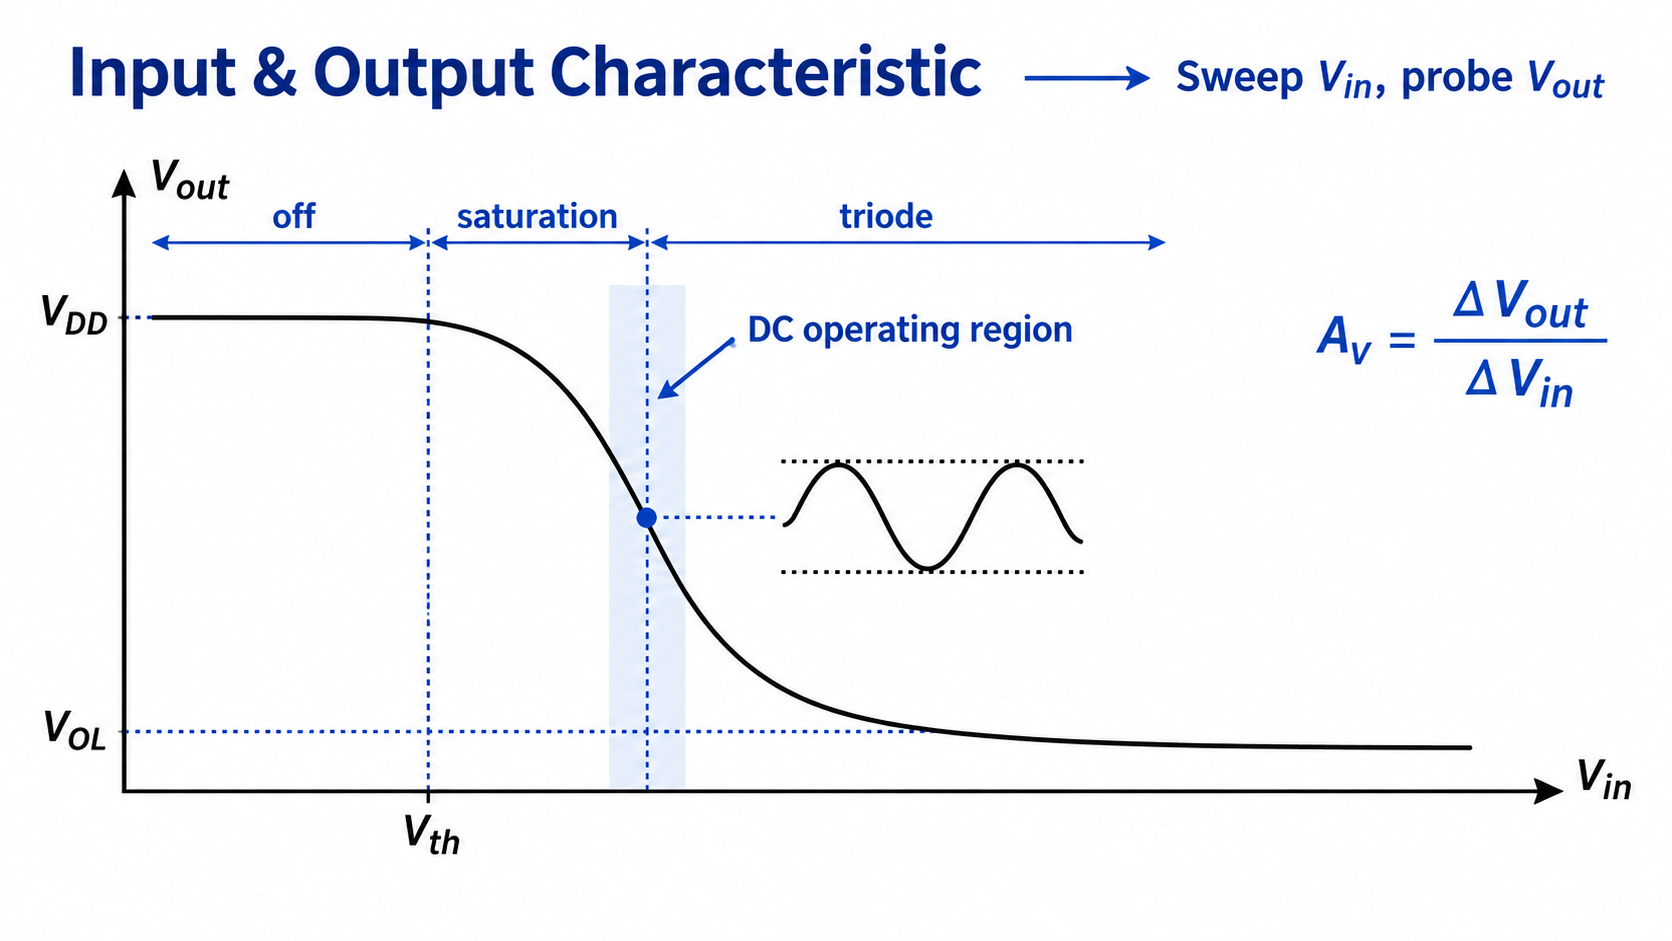
\includegraphics[width=0.8\linewidth]{figures/input-output-characteristic.png}
    \caption{Voltage Transfer Characteristic of a Common-Source Amplifier with Resistive Load}
    \label{fig:cs-amplifier-characteristic}
\end{figure}

\Needspace{45mm}
In deep triode, with $V_{\mathrm{out}} \ll V_{OV}$, the transistor acts approximately as a gate-controlled resistor.
\begin{notecircuit}[american, scale=0.7, transform shape]{Deep-Triode Equivalent: $M_1$ as a Resistor}
    % R_DS represents the drain--source resistance of M1 at its gate bias.
    \coordinate (out) at (0,1.2);
    \draw (out) to[R,l=$R_{DS}$] (0,-1.2) node[ground] {};

    % Preserve the drain load, supply, and output from the previous circuit.
    \draw (out) to[R,l=$R_D$] ++(0,1.3)
    -- ++(0,0.25) node[vcc] {$V_{DD}$};
    \draw (out) node[circ] {} -- ++(1.1,0)
    node[ocirc] {} node[right] {$V_{\mathrm{out}}$};
\end{notecircuit}
\subnotesection{Determining Gain: Small-Signal Model of the CS Amplifier}
\assumption{The transistor is biased in saturation. The low-frequency model neglects capacitances and body effect.}

\Needspace{45mm}
\begin{notecircuit}[american, scale=0.7, transform shape]{Common-Source Small-Signal Equivalent}
    % The gate draws no current; v_gs is measured relative to the grounded source.
    \draw (-4,0) node[ground] {}
    to[sV,l_=$v_{\mathrm{in}}$] (-4,2)
    -- (-2.5,2) node[ocirc] {} node[above] {$G$};
    \draw (-2.5,0) node[ocirc] {} -- (0,0);
    \node at (-2.2,1.75) {$+$};
    \node at (-2.2,0.25) {$-$};
    \node at (-1.85,1) {$v_{gs}$};

    % Drain-to-source controlled current and transistor output resistance.
    \draw (0,2) to[cI,l=$g_m v_{gs}$] (0,0)
    node[circ] {} node[below left] {$S$} node[ground] {};
    \draw (0,2) node[circ] {} -- (2,2)
    node[circ] {} node[above] {$D$}
    to[R,l=$r_o$] (2,0) -- (0,0);

    % The DC supply becomes AC ground at the far end of R_D.
    \draw (2,2) -- (4,2) coordinate (load)
        to[R,l=$R_D$] (4,0) node[ground] {};
    \draw (load) node[circ] {} -- ++(0.9,0)
    node[ocirc] {} node[right] {$v_{\mathrm{out}}$};
    \node[right,align=left,font=\small,text=NoteMuted] at (4.3,0)
    {$V_{DD}$\\AC ground};
    \node[text=NoteAccent] at (2,-0.9) {$R_L = r_o \parallel R_D$};
\end{notecircuit}

\begin{notederivation}{Gain, $A_V$, of a CS Amplifier}
    & A_V = \frac{v_{\mathrm{out}}}{v_{\mathrm{in}}} && \quad \text{Definition of gain} \\
    & \frac{v_{\mathrm{out}}}{R_D} + \frac{v_{\mathrm{out}}}{r_o} + g_m v_{gs} = 0
    && \quad \text{KCL at the drain} \\
    & v_{\mathrm{out}} = -g_m v_{gs}(r_o \parallel R_D)
    && \quad v_{gs} = v_{\mathrm{in}} \\
    & v_{\mathrm{out}} = -g_m v_{\mathrm{in}}(r_o \parallel R_D)
\end{notederivation}

\keyequation{Gain of a CS Amplifier}{A_V = \frac{v_{\mathrm{out}}}{v_{\mathrm{in}}} = -g_m (r_o \parallel R_D)}

\Needspace{75mm}
\notesection{CS Amplifier with Diode-Connected Load}


\Needspace{40mm}
\begin{notecircuit}[american, scale=0.7, transform shape]{CS Amplifier with NMOS Diode-Connected Load}
    \draw (0,0) node[nmos,arrowmos] (M1) {$M_1$};
    \draw (0,1.8) node[nmos,arrowmos] (M2) {$M_2$};

    % Input transistor: gate input and grounded source.
    \draw (M1.G) -- ++(-1.1,0)
    node[ocirc] {} node[left] {$V_{\mathrm{in}}$};
    \draw (M1.S) -- ++(0,-0.5) node[ground] {};

    % The output joins M1's drain to M2's source.
    \draw (M1.D) -- (M2.S) coordinate[midway] (out);
    \draw (out) node[circ] {} -- ++(1.1,0)
    node[ocirc] {} node[right] {$V_{\mathrm{out}}$};

    % Diode-connected load: M2's gate and drain are tied to V_DD.
    \draw (M2.D) -- ++(0,0.35) coordinate (supply)
        node[vcc] {$V_{DD}$};
    \draw (M2.G) -- ++(-0.35,0) coordinate (gate-link)
        -- (gate-link |- supply) -- (supply) node[circ] {};
\end{notecircuit}
\begin{itemize}
    \item Tying the drain to the gate gives $V_{GS2} = V_{DS2}$. When conducting, $M_2$ is in the \textcolor{red}{saturation} region.
    \item Ignoring body effect, the small-signal resistance is $r_{eq} = \frac{1}{g_{m2}} \parallel r_{o2}$.
          When $g_{m2}r_{o2} \gg 1$, this reduces to $r_{eq} \approx \frac{1}{g_{m2}}$.
\end{itemize}

\Needspace{40mm}
To determine $r_{eq} = V_x/I_x$, apply a small test voltage $V_x$ about a bias point where $M_2$ is conducting.
\begin{notecircuit}[american, scale=0.7, transform shape]{Diode-Connected NMOS with a Test Source}
    \draw (0,0) node[nmos,arrowmos] (M2) {$M_2$};
    \draw (M2.D) -- ++(0,0.35) coordinate (drain) node[circ] {};
    \draw (M2.S) -- ++(0,-0.35) coordinate (source);

    % Tie the gate to the drain, so V_GS = V_DS = V_x.
    \draw (M2.G) -- ++(-0.35,0) coordinate (gate-link)
    -- (gate-link |- drain) -- (drain);

    % Positive test voltage at the drain; I_x flows into the transistor.
    \coordinate (test) at (1.8,0);
    \draw[color=orange!80!black] (test |- drain) to[short,i=$I_x$] (drain);
    \draw[color=NoteAccent] (test |- drain)
    to[american voltage source,l=$V_x$] (test |- source)
    -- (source);
\end{notecircuit}
\notedefinition{PMOS Small Signal}{
    The small signal model of a PMOS is equivalent to a NMOS circuit
}

\Needspace{95mm}
\notesection{CS with Current-Source Load}

\begin{notecircuit}[american, scale=0.7, transform shape]{CS Amplifier with a PMOS Current-Source Load}
    \draw (0,0) node[nmos,arrowmos] (M1) {$M_1$};
    \draw (0,1.8) node[pmos,arrowmos] (M2) {$M_2$};

    % NMOS input stage and fixed PMOS gate bias.
    \draw (M1.G) -- ++(-1.1,0)
    node[ocirc] {} node[left] {$V_{\mathrm{in}}$};
    \draw (M1.S) -- ++(0,-0.5) node[ground] {};
    \draw (M2.G) -- ++(-1.1,0)
    node[ocirc] {} node[left] {$V_B$};
    \draw (M2.S) -- ++(0,0.35) node[vcc] {$V_{DD}$};

    % The two drains meet at the output.
    \draw (M1.D) -- (M2.D) coordinate[midway] (out);
    \draw (out) node[circ] {} -- ++(1.1,0)
    node[ocirc] {} node[right] {$V_{\mathrm{out}}$};
\end{notecircuit}
\begin{itemize}
    \item Since $V_B$ and $V_{DD}$ is a DC power source, we can treat it as a open circuit and assume that $V_{SG} = V_{DD} - V_{B} = 0 \therefore g_{m2}V_{sg2} = 0$
\end{itemize}
\Needspace{40mm}
\begin{notecircuit}[american, scale=0.7, transform shape]{Small-Signal Equivalent: $v_{sg2} = 0$}
    % The NMOS gate input is measured relative to its grounded source.
    \draw (-4,0) node[ground] {}
    to[sV,l_=$v_{\mathrm{in}}$] (-4,2)
    -- (-2.5,2) node[ocirc] {} node[above] {$G$};
    \draw (-2.5,0) node[ocirc] {} -- (0,0);
    \node at (-2.2,1.75) {$+$};
    \node at (-2.2,0.25) {$-$};
    \node at (-1.85,1) {$v_{gs1}$};

    % M1's transconductance source and output resistance.
    \draw (0,2) to[cI,l=$g_{m1}v_{gs1}$] (0,0)
    node[circ] {} node[ground] {};
    \draw (0,2) node[circ] {} -- (2.4,2)
    node[circ] {} to[R,l=$r_{o1}$] (2.4,0) -- (0,0);

    % V_B and V_DD are AC grounds, so M2 contributes only r_o2.
    \draw (2.4,2) -- (4.4,2) coordinate (out)
        to[R,l=$r_{o2}$] (4.4,0) -- (2.4,0) node[circ] {};
    \draw (out) node[circ] {} -- ++(0.9,0)
    node[ocirc] {} node[right] {$v_{\mathrm{out}}$};
\end{notecircuit}
\notesection{Cascode with Ideal Source}
\begin{figure}[htbp]
    \centering
    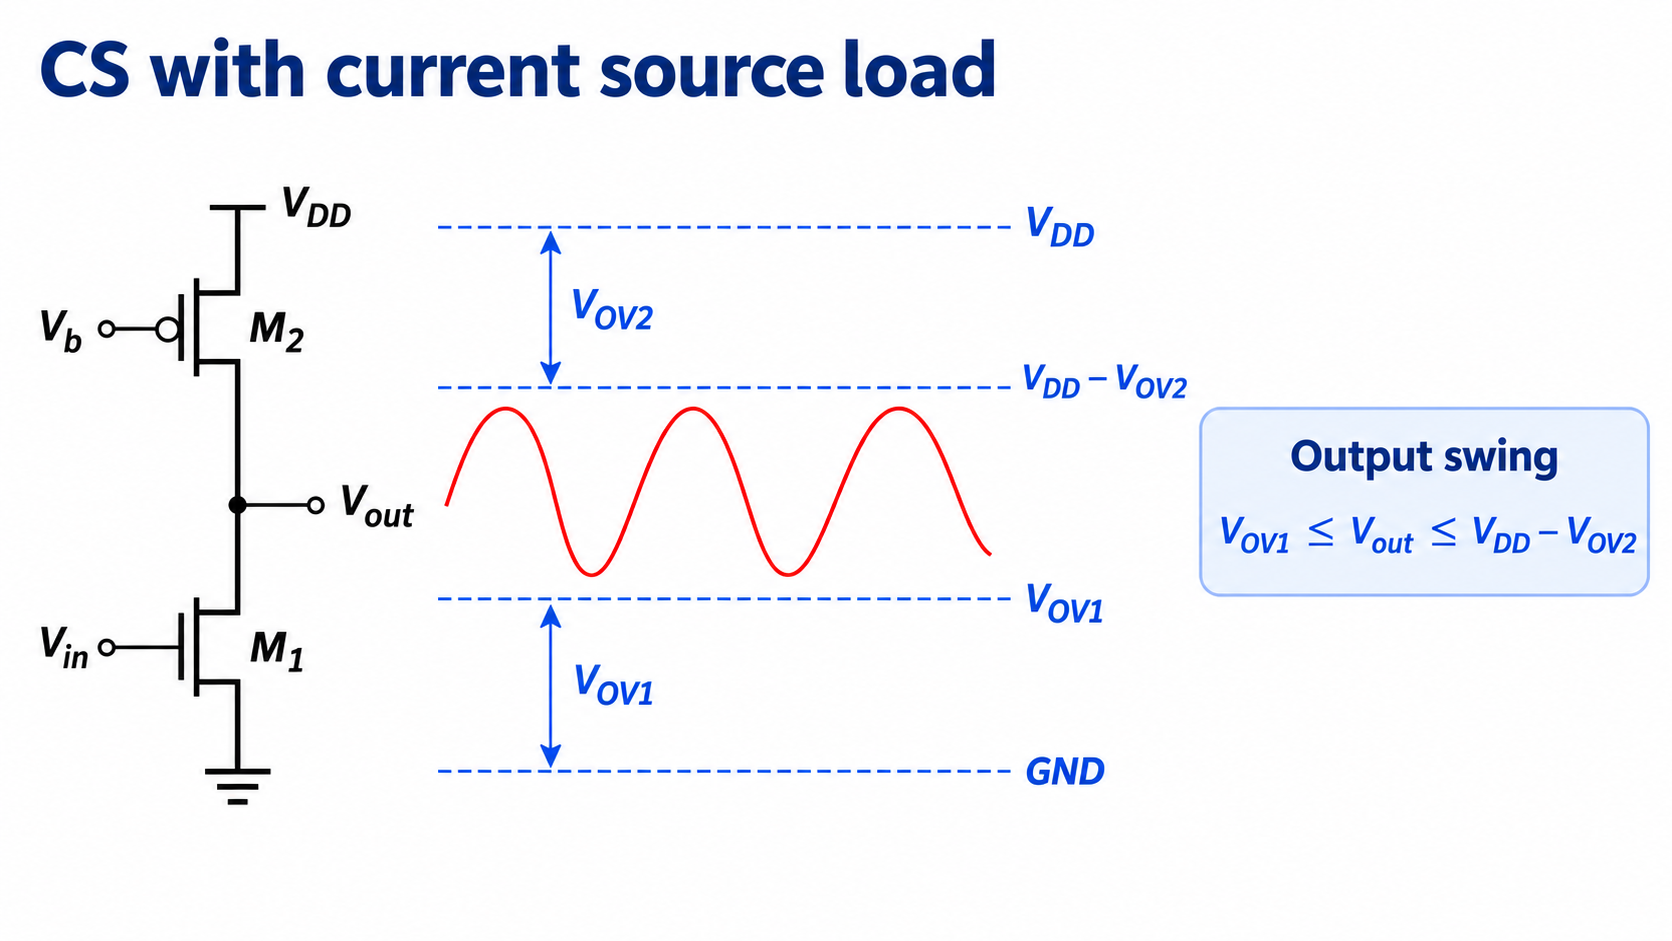
\includegraphics[width=0.6\linewidth]{figures/cs-current-source-load-output-swing.png}
    \caption{CS Amp with Current Source Output Swing}
    \label{fig:}
\end{figure}

\keyequation{Gain of a CS Amplifier with a Current Source Load}{A_V = g_{m1} (r_{o1} || r_{o2})}[Note that $g_{m2}$ is proportional to $I_d$ or $\frac{W}{L}$]

\Needspace{72mm}
\notesection{Increasing the Gain of a Single Stage Amp}
\begin{figure}[htbp]
    \centering
    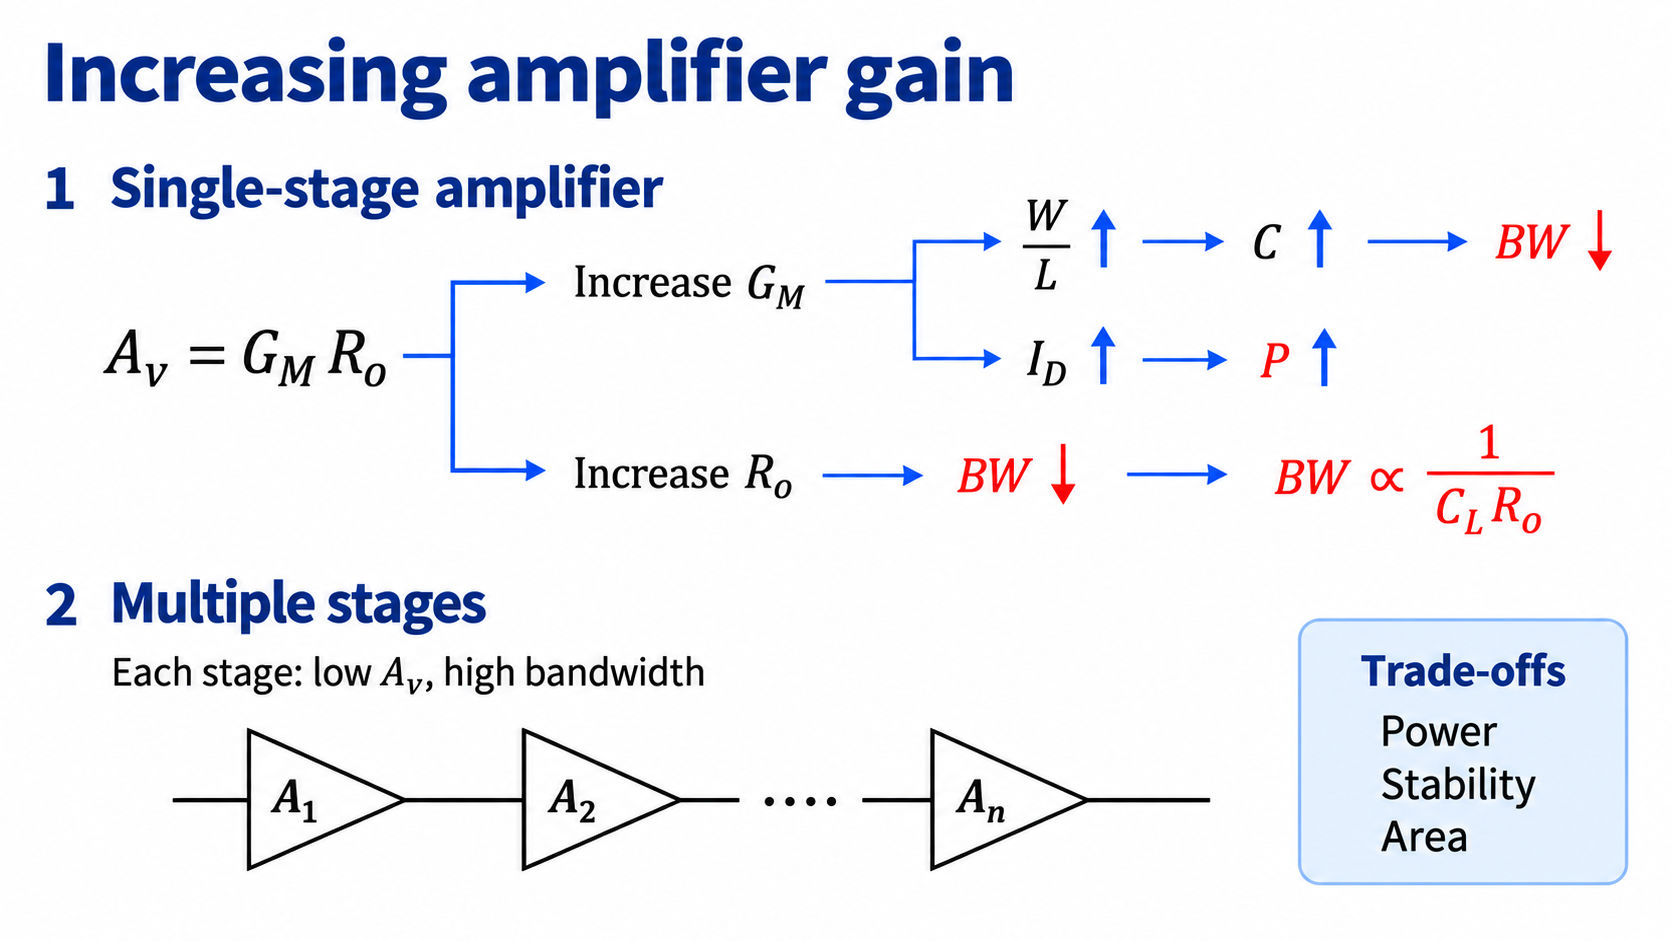
\includegraphics[width=0.6\linewidth]{figures/amplifier-gain-single-vs-multistage.png}
    \caption{Amplifier Gain Single vs. Multi Stage}
    \label{fig:}
\end{figure}

Increasing the gain of a multi-stage amplifier comes with less trade-offs and is less complex than a single stage ampliifer

\notesection{Norton's Theorem}

\begin{figure}[htbp]
    \centering
    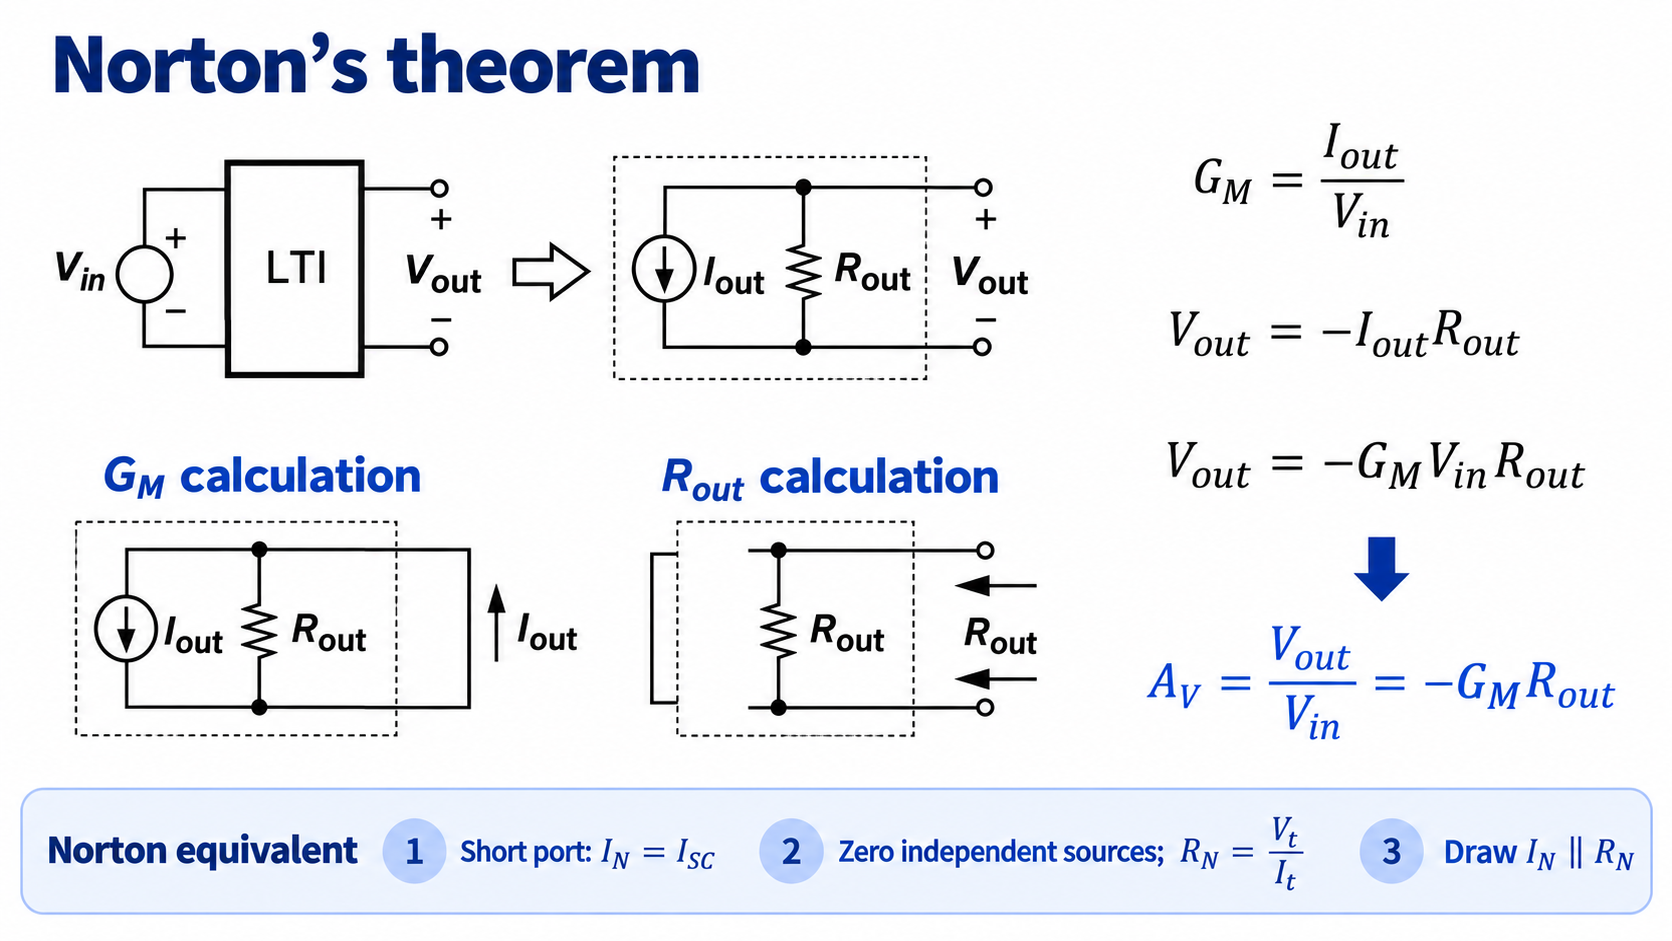
\includegraphics[width=0.6\linewidth]{figures/norton-theorem-small-signal-amplifier.png}
    \caption{Nortons Theorem Small-Signal Equivalent Application}
    \label{fig:}
\end{figure}


\notesection{Cascode with Ideal Source}

\begin{notecircuit}[american, scale=0.55, transform shape]{Cascode with an Ideal Current Source}
    \draw (0,0) node[nmos,arrowmos] (M1) {$M_1$};
    \draw (0,1.65) node[nmos,arrowmos] (M2) {};

    \draw (M1.G) -- ++(-0.65,0)
        node[ocirc] {} node[left] {$V_{\mathrm{in}}$};
    \draw (M1.S) -- ++(0,-0.35) node[ground] {};
    \draw (M1.D) -- (M2.S);
    \draw (M2.G) -- ++(-0.65,0)
        node[ocirc] {} node[left] {$V_B$};
    \node[above right, inner sep=1pt] at (M2.bulk) {$M_2$};
    % M2's body is grounded; keep this connection distinct from the signal path.
    \draw[violet!75!black, densely dashed] (M2.bulk) -- ++(1.0,0)
        node[ground, color=violet!75!black] {}
        node[right, color=violet!75!black] {$V_{B2}$};

    \draw (M2.D) -- ++(0,0.3) coordinate (out);
    \draw (out) node[circ] {} -- ++(0.7,0)
        node[ocirc] {} node[right] {$V_{\mathrm{out}}$};
    \draw (0,4.9) node[vcc] {$V_{DD}$} -- (0,4.65)
        to[I,l_=$I_1$] (0,3.6) -- (out);
\end{notecircuit}

\assumption{
    \begin{itemize}
        \item Body is connected to ground
        \item The ideal current source is an open circuit in the small-signal model.
        \item $\lambda \neq 0$ makes $r_o$ finite, and $\gamma \neq 0$ gives M2 a body-effect current source $g_{mb2}v_{bs2}$ between nodes B and A.
        \item Looking at the original circuit, with the gate and body of M2 at AC ground:
        \begin{itemize}
            \item $v_{\mathrm{in}} = v_{gs1}$
            \item $v_{gs2} = 0 - v_A = -v_A$
            \item $v_{bs2} = 0 - v_A = -v_A$
        \end{itemize}
    \end{itemize}
}

\Needspace{70mm}
\begin{notecircuit}[american, scale=0.55, transform shape]{Cascode Small-Signal Equivalent with Body Effect}
    \coordinate (A) at (0,2);
    \coordinate (B) at (0,5);

    % M1: an open gate, transconductance source, and output resistance.
    \draw (-6.4,0) node[ground] {}
        to[sV,l_=$v_{\mathrm{in}}$] (-6.4,2)
        -- (-5.1,2) node[ocirc] {};
    \draw (-5.1,0) node[ocirc] {} -- (0,0);
    \node at (-4.8,1.75) {$+$};
    \node at (-4.8,0.25) {$-$};
    \node at (-4.1,1) {$v_{gs1}$};
    \draw (A) to[cI,l_=$g_{m1}v_{gs1}$] (0,0) node[ground] {};
    \draw (A) -- (2.3,2) to[R,l=$r_{o1}$] (2.3,0) -- (0,0);

    % M2's gate bias becomes AC ground; its source is node A.
    \draw (-4.0,5) node[ground] {} -- (-3.3,5) node[ocirc] {};
    \draw (-3.3,2) node[ocirc] {} -- (A);
    \node at (-3.0,4.7) {$+$};
    \node at (-3.0,2.3) {$-$};
    \node at (-2.4,3.5) {$v_{gs2}$};
    \draw (B) to[cI,l=$g_{m2}v_{gs2}$] (A);
    \draw (B) -- (2.3,5) to[R,l=$r_{o2}$] (2.3,2);

    % The body is also AC-grounded; its control voltage is measured to A.
    \draw (2.3,5) -- (5.0,5) -- (5.8,5)
        node[ocirc] {} node[right] {$v_{\mathrm{out}}$};
    \draw[violet!75!black] (5.0,5)
        to[cI,l=$g_{mb2}v_{bs2}$] (5.0,2);
    \draw (5.0,2) -- (A);
    \draw[violet!75!black] (7.2,5) node[ground] {}
        -- (7.2,4.7) node[ocirc] {};
    \draw[violet!75!black] (7.2,2) node[ocirc] {} -- (5.0,2);
    \node[violet!75!black] at (7.55,4.4) {$+$};
    \node[violet!75!black] at (7.55,2.3) {$-$};
    \node[violet!75!black, right] at (7.7,3.5) {$v_{bs2}$};

    % Highlight the two internal nodes used in the small-signal analysis.
    \fill[red] (A) circle (2pt);
    \node[red, above left] at (A) {$A$};
    \fill[red] (2.3,5) circle (2pt);
    \node[red, above] at (2.3,5) {$B$};
\end{notecircuit}

\subnotesection{Finding $G_M$ through small-signal analysis}
For the short-circuit transconductance, set $v_B = v_{\mathrm{out}} = 0$ and define
$i_{\mathrm{out}}$ as entering node B from the output short.
\begin{notederivation}{Finding $G_M$}
    & i_{\mathrm{out}} = g_{m1}v_{\mathrm{in}} + \frac{v_A}{r_{o1}}
    && \quad \text{KCL at A} \\
    & i_{\mathrm{out}} = g_{m2}v_{gs2} + g_{mb2}v_{bs2} - \frac{v_A}{r_{o2}}
    && \quad \text{KCL at B} \\
    & i_{\mathrm{out}} = -v_A\left(g_{m2}+g_{mb2}+\frac{1}{r_{o2}}\right)
    && \quad v_{gs2}=v_{bs2}=-v_A \\
    & i_{\mathrm{out}} = g_{m1}v_{\mathrm{in}}
      - \frac{i_{\mathrm{out}}}{r_{o1}\left(g_{m2}+g_{mb2}+1/r_{o2}\right)}
    && \quad \text{substitute into KCL at A} \\
    & G_M \equiv \frac{i_{\mathrm{out}}}{v_{\mathrm{in}}}
      = \frac{g_{m1}}{1+\dfrac{1}{r_{o1}\left(g_{m2}+g_{mb2}+1/r_{o2}\right)}}
    && \quad \text{solve for }i_{\mathrm{out}} \\
    & G_M \approx g_{m1}\frac{1.3g_{m2}r_{o1}}{1+1.3g_{m2}r_{o1}}
    && \quad g_{mb2}\approx0.3g_{m2},\;r_{o2}\text{ large} \\
    & G_M \approx g_{m1}
    && \quad 1.3g_{m2}r_{o1}\gg1
\end{notederivation}

\Needspace{185mm}
\subnotesection{Nortons to find $R_o$}
\assumption{\begin{itemize}
    \item $V_{in} = 0 \therefore g_{m1}V_{in} = 0$
    \item $V_b = 0$
    \item $V_{dd} = 0$
\end{itemize}}

\begin{notecircuit}[american, scale=0.55, transform shape]{Norton Small-Signal Equivalent for Finding $R_o$}
    \coordinate (A) at (0,2);
    \coordinate (B) at (0,5);

    % M1's transconductance source vanishes when the input is zero.
    \draw (A) to[R,l=$r_{o1}$] (0,0) node[ground] {};

    % M2's gate is AC-grounded; its source remains at node A.
    \draw (-4.0,5) node[ground] {} -- (-3.3,5) node[ocirc] {};
    \draw (-3.3,2) node[ocirc] {} -- (A);
    \node at (-3.0,4.7) {$+$};
    \node at (-3.0,2.3) {$-$};
    \node at (-2.4,3.5) {$v_{gs2}$};
    \draw (B) to[cI,l=$g_{m2}v_{gs2}$] (A);
    \draw (B) -- (2.3,5) to[R,l=$r_{o2}$] (2.3,2) -- (A);

    % Retain M2's body effect, using the same violet as its body connection.
    \draw (2.3,5) -- (5.0,5);
    \draw[color=violet!75!black] (5.0,5)
        to[cI,l=$g_{mb2}v_{bs2}$] (5.0,2);
    \draw (5.0,2) -- (A);
    \node[color=violet!75!black, below] at (5.0,1.8) {$v_{bs2}=-v_A$};

    % Apply the test voltage at B; I_X enters the circuit from the test source.
    \draw[color=orange!80!black] (8.6,5)
        to[short,i=$I_X$] (5.0,5);
    \draw[color=orange!80!black] (8.6,5)
        to[american voltage source,l=$V_X$] (8.6,2) node[ground] {};

    \fill[red] (A) circle (2pt);
    \node[red, above left] at (A) {$A$};
    \fill[red] (2.3,5) circle (2pt);
    \node[red, above] at (2.3,5) {$B$};
\end{notecircuit}

\begin{notederivation}{Finding $R_o$ from the Norton Test Circuit}
    & I_X = g_{m2}v_{gs2} + g_{mb2}v_{bs2}
      + \frac{V_X-v_A}{r_{o2}}
    && \quad \text{KCL at B} \\
    & v_{gs2}=v_{bs2}=-v_A,\qquad v_A=I_Xr_{o1}
    && \quad \text{AC grounds and KCL at A} \\
    & I_X = -g_{m2}v_A-g_{mb2}v_A
      + \frac{V_X}{r_{o2}}-\frac{v_A}{r_{o2}}
    && \quad \text{substitute control voltages} \\
    & I_X = -I_Xr_{o1}\left(g_{m2}+g_{mb2}+\frac{1}{r_{o2}}\right)
      + \frac{V_X}{r_{o2}}
    && \quad \text{substitute }v_A \\
    & I_X\left(1+g_{m2}r_{o1}+g_{mb2}r_{o1}+\frac{r_{o1}}{r_{o2}}\right)
      = \frac{V_X}{r_{o2}}
    && \quad \text{collect }I_X \\
    & R_o \equiv \frac{V_X}{I_X}
      = g_{m2}r_{o1}r_{o2}+g_{mb2}r_{o1}r_{o2}+r_{o1}+r_{o2}
    && \quad \text{output resistance} \\
    & R_o \approx (g_{m2}+g_{mb2})r_{o1}r_{o2}
    && \quad \text{dominant cascode term}
\end{notederivation}

With the input restored, the Norton current is $i_{\mathrm{out}}=G_Mv_{\mathrm{in}}$,
and $v_{\mathrm{out}}=-i_{\mathrm{out}}R_o$ using the current direction defined above.

\keyequation{Voltage Gain of the Cascode Amplifier}{
    A_V \equiv \frac{v_{\mathrm{out}}}{v_{\mathrm{in}}}
    = -G_MR_o
    \approx -g_{m1}r_{o1}(g_{m2}+g_{mb2})r_{o2}
}[Using $G_M\approx g_{m1}$ and neglecting $r_{o1}+r_{o2}$ when
$(g_{m2}+g_{mb2})r_{o1}r_{o2}\gg r_{o1}+r_{o2}$.]

\notesection{Source Follow \& Common Gate Amplifiers}

\begin{figure}[htbp]
    \centering
    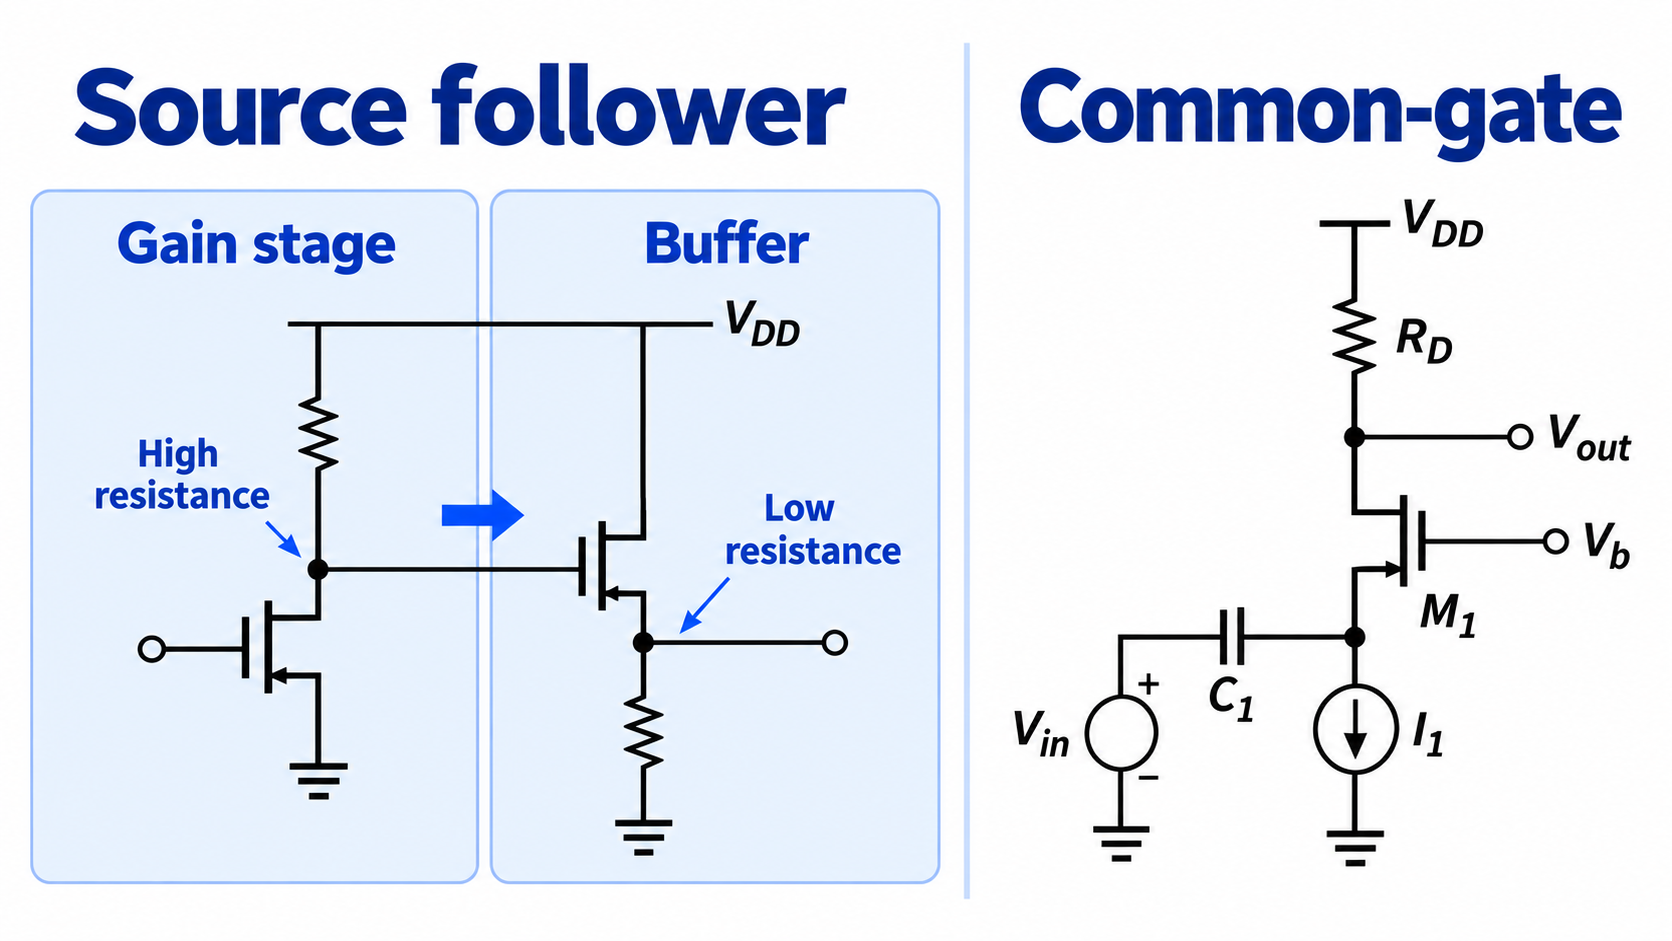
\includegraphics[width=0.8\linewidth]{figures/source-follower-vs-common-gate.png}
    \caption{Source Follower and Common-Gate Configuration}
    \label{fig:}
\end{figure}

\end{document}
